\documentclass[a4paper,12pt,notitlepage,oneside]{book}

% \linespread{1.3}

\usepackage[T1]{fontenc}
\usepackage[magyar]{babel}
\usepackage[utf8x]{inputenc}
\usepackage{url}
\usepackage{subfig}
\usepackage[abs]{overpic}
\usepackage{enumerate}
\usepackage{datetime}

\usepackage{pgf}
\usepackage{tikz}
\usetikzlibrary{positioning}
\usetikzlibrary{patterns}
\usetikzlibrary{decorations.pathreplacing}
\usetikzlibrary{scopes,arrows}
\usetikzlibrary{decorations.markings}
% \usepackage{tikz-3dplot}

\frenchspacing
\usepackage{icomma}
\usepackage{indentfirst}

\usepackage{amssymb}
\usepackage{amsmath}
\usepackage{fancyhdr}
\usepackage{fullpage}
% \usepackage[margin=2cm]{geometry}
\usepackage[top=1.8cm, bottom=2.2cm, left=2.25cm, right=2.25cm]{geometry}
% \usepackage[top=1.8cm, bottom=2.2cm, left=2.5cm, right=2cm]{geometry}


\usepackage{array}
\usepackage{graphicx}

\allowdisplaybreaks[1]

\newcommand{\eqaref}[1]{\az+\eqref{#1}}
\newcommand{\Eqaref}[1]{\Az+\eqref{#1}}

\newcommand{\ce}[3]{{_{#1}^{#2}}\mathrm{#3}}

%%%%%%%%% Numbering %%%%%%%%%%%%%
\numberwithin{equation}{chapter}   %Equation numbering
\numberwithin{chapter}{part}   %chapter numbering
\numberwithin{section}{chapter}   %chapter numbering
\numberwithin{subsection}{section}   %chapter numbering
\addto\captionsmagyar{\renewcommand{\chaptername}{t\'etel}} %Change ``#. fejezet'' to ``#. tétel''
\addto\captionsmagyar{\renewcommand{\partname}{t\'etelek}} %Change ``#. fejezet'' to ``#. tétel''
\renewcommand\thechapter{\Alph{part}-\arabic{chapter}} %Change the chapter numbering ``chapternumber'' to ``partnumber-chapternumber'' where partnumber is like A, B, C, ...
\renewcommand\thepart{\Alph{part}} %Change ``chapternumber'' to A, B, C, ...
\usepackage{tocstyle}   %Package to calculate space for chapter numbering in TOC.
\usetocstyle{standard}
\usepackage{titlesec}

\usepackage{multirow}
\usepackage{pdflscape}
% \usepackage{bookmark}

\newtheorem{feladat}{feladat}
\newcommand{\me}[1]{\mathrm{\, #1}}

\newcommand{\dd}{\mathrm{d}}
\newcommand{\ep}{\varepsilon}
\newcommand{\mbf}{\mathbf}
\newcommand{\tg}{\mathop{\mathrm{tg}}\nolimits}
\newcommand{\ctg}{\mathop{\mathrm{ctg}}\nolimits}
\renewcommand{\Im}{\mathop{\mathrm{Im}}\nolimits}
\renewcommand{\Re}{\mathop{\mathrm{Re}}\nolimits}
\newcommand{\arctg}{\mathop{\mathrm{arctg}}\nolimits}
\newcommand{\tr}{\mathop{\mathrm{Tr}}\nolimits}
\newcommand{\sh}{\mathop{\mathrm{sh}}\nolimits}
\newcommand{\tgh}{\mathop{\mathrm{th}}\nolimits}
\newcommand{\ctgh}{\mathop{\mathrm{cth}}\nolimits}
\newcommand{\arcth}{\mathop{\mathrm{arcth}}\nolimits}
\newcommand{\ch}{\mathop{\mathrm{ch}}\nolimits}
\newcommand{\sgn}{\mathop{\mathrm{sgn}}\nolimits}
\newcommand{\intdom}{\mathop{\mathrm{int}}\nolimits}

\newcommand{\grad}{\mathop{\vects{\nabla}}\nolimits}
\providecommand{\divo}{\mathop{\vects{\nabla}}\nolimits}
\providecommand{\rot}{\mathop{\vects{\nabla}\times}\nolimits}

\newcommand{\Lin}{\mathop{\mathrm{Lin}}\nolimits}
\newcommand{\T}{\mathop{\mathrm{T}}\nolimits}


\providecommand{\abs}[1]{\left\lvert#1\right\rvert}
\providecommand{\norm}[1]{\lVert#1\rVert}
\providecommand{\bra}[1]{\langle#1\rvert}
\providecommand{\ket}[1]{\lvert#1\rangle}
\providecommand{\et}[1]{#1\rangle}
\providecommand{\mv}[1]{\left\langle#1\right\rangle}

\providecommand{\eq}[1]{\begin{equation*} #1 \end{equation*}}
\providecommand{\eqn}[1]{\begin{equation} #1 \end{equation}}

\providecommand{\al}[1]{\begin{align*} #1 \end{align*}}
\providecommand{\aln}[1]{\begin{align} #1 \end{align}}

\providecommand{\der}[2]{\frac{\dd #1}{\dd #2}}
\providecommand{\pder}[2]{\frac{\partial #1}{\partial #2}}
\providecommand{\suml}[2]{\sum\limits_{#1}^{#2}}
\providecommand{\prodl}[2]{\prod\limits_{#1}^{#2}}
\providecommand{\intl}[2]{\int\limits_{#1}^{#2}}
\providecommand{\ointl}[2]{\oint\limits_{#1}^{#2}}

\newcommand{\ddtx}{\ddot{x}}
\newcommand{\dtx}{\dot{x}}
\newcommand{\ddtq}{\ddot{q}}
\newcommand{\dtq}{\dot{q}}
\newcommand{\dtp}{\dot{p}}
\newcommand{\ddtQ}{\ddot{Q}}
\newcommand{\dtQ}{\dot{Q}}
\newcommand{\dtP}{\dot{P}}

\newcommand{\dtr}{\dot{\vect{r}}}
\newcommand{\ddtr}{\ddot{\vect{r}}}

\newcommand{\Av}{\vect{A}}
\newcommand{\av}{\vect{a}}
\newcommand{\Bv}{\vect{B}}
\newcommand{\bv}{\vect{b}}
\newcommand{\Dv}{\vect{D}}
\newcommand{\ev}{\vect{e}}
\newcommand{\Ev}{\vect{E}}
\newcommand{\Fv}{\vect{F}}
\newcommand{\fv}{\vect{f}}
\newcommand{\gv}{\vect{g}}
\newcommand{\Gv}{\vect{G}}
\newcommand{\Hv}{\vect{H}}
\newcommand{\hv}{\vect{h}}
\newcommand{\Jv}{\vect{J}}
\newcommand{\jv}{\vect{j}}
\newcommand{\kv}{\vect{k}}
\newcommand{\lv}{\vect{l}}
\newcommand{\Lv}{\vect{L}}
\newcommand{\Mv}{\vect{M}}
\newcommand{\emv}{\vect{m}}
\newcommand{\nv}{\vect{n}}
\newcommand{\pv}{\vect{p}}
\newcommand{\Pv}{\vect{P}}
\newcommand{\qv}{\vect{q}}
\newcommand{\rv}{\vect{r}}
\newcommand{\Rv}{\vect{R}}
\newcommand{\Sv}{\vect{S}}
\newcommand{\sv}{\vect{s}}
\newcommand{\uv}{\vect{u}}
\newcommand{\vv}{\vect{v}}
\newcommand{\xv}{\vect{x}}
\newcommand{\Xv}{\vect{X}}

\newcommand{\alv}{\vects{\alpha}}
\newcommand{\betav}{\vects{\beta}}
\newcommand{\gammav}{\vects{\gamma}}
\newcommand{\muv}{\vects{\mu}}
\newcommand{\Piv}{\vects{\Pi}}
\newcommand{\sigv}{\vects{\sigma}}
\newcommand{\omv}{\vects{\omega}}


\newcommand{\oprv}{\op{\vect{r}}}
\newcommand{\opvv}{\op{\vect{v}}}
\newcommand{\oppv}{\op{\vect{p}}}
\newcommand{\opLv}{\op{\vect{L}}}
\newcommand{\opav}{\op{\vect{a}}}
\newcommand{\opkv}{\op{\vect{k}}}


\newcommand{\opA}{\op{A}}
\newcommand{\opa}{\op{a}}
\newcommand{\opad}{\op{a}^\dagger}
\newcommand{\opB}{\op{B}}
\newcommand{\opC}{\op{C}}
\newcommand{\opH}{\op{H}}
\newcommand{\opG}{\op{G}}
\newcommand{\opI}{\op{I}}
\newcommand{\opL}{\op{L}}
\newcommand{\opN}{\op{N}}
\newcommand{\opp}{\op{p}}
\newcommand{\opr}{\op{r}}
\newcommand{\opR}{\op{R}}
\newcommand{\opS}{\op{S}}
\newcommand{\opT}{\op{T}}
\newcommand{\opV}{\op{V}}
\newcommand{\opx}{\op{x}}
\newcommand{\opX}{\op{X}}
\newcommand{\opy}{\op{y}}
\newcommand{\opY}{\op{Y}}
\newcommand{\opSv}{\op{\vect{S}}}

\newcommand{\opmuv}{\op{\vects{\mu}}}
\newcommand{\opsigv}{\op{\vects{\sigma}}}



% \providecommand{\brapsii}{\langle\psi_i\rvert}
% \newcommand{\ketpsii}{\lvert\psi_i\rangle}
% \newcommand{\econr}{\vect{e}_\text{con}(\vect{r})}
% \newcommand{\bconr}{\vect{B}_\text{con}(\vect{r})}
% \newcommand{\bxcr}{\vect{B}_\text{xc}(\vect{r})}
% \newcommand{\evecr}{\vect{e}(\vect{r})}
% \newcommand{\cvecr}{\vect{c}(\vect{r})}
% \newcommand{\econ}{\vect{e}_\text{con}}
% \newcommand{\bcon}{\vect{B}_\text{con}}
% \newcommand{\evec}{\vect{e}}
% \newcommand{\cvec}{\vect{c}}
% \newcommand{\psig}{\boldsymbol{\sigma}}
% \newcommand{\pSig}{\boldsymbol{\Sigma}}
% \newcommand{\palpha}{\boldsymbol{\alpha}}
% 
% \providecommand{\spsiir}{\ket{\psi_i(\vect{r})}}
% \providecommand{\spsiipr}{\bra{\psi_i(\vect{r})}}
% \providecommand{\psiir}{\psi_i(\vect{r})\rangle}
% \providecommand{\spsikr}{\ket{\psi_k(\vect{r})}}
% \providecommand{\spsikpr}{\bra{\psi_k(\vect{r})}}
% \providecommand{\psikr}{\psi_k(\vect{r})\rangle}
% \providecommand{\nur}{n_\uparrow(\vect{r})}
% \providecommand{\ndr}{n_\downarrow(\vect{r})}

\providecommand{\vect}[1]{\mathbf{#1}}
\providecommand{\vects}[1]{\boldsymbol{#1}}
\providecommand{\mat}[1]{\underline{\underline{#1}}}
\providecommand{\minv}[1]{\mathsf{#1}}
\providecommand{\ominv}[1]{\op{\mathsf{#1}}}

\providecommand{\op}[1]{\hat{#1}}
\newcommand{\drh}{\dd^3\vect{r}\,}
\newcommand{\drkh}{\dd^3\vect{r'}\,}
\newcommand{\df}{\dd^2\vect{f}\,}
\newcommand{\ds}{\dd^2\vect{s}\,}
\newcommand{\ddt}{\dd t\,}
\newcommand{\drv}{\dd \rv\,}
\newcommand{\TC}{T_\text{C}}
\newcommand{\kB}{k_\text{B}}

\usepackage{hyperref}
\hypersetup{
%     bookmarks=true,         % show bookmarks bar?
    unicode=true,          % non-Latin characters in Acrobat’s bookmarks
%     pdftoolbar=false,        % show Acrobat’s toolbar?
%     pdfmenubar=true,        % show Acrobat’s menu?
%     pdffitwindow=false,     % window fit to page when opened
%     pdfstartview={FitH},    % fits the width of the page to the window
%     pdfcenterwindow={true}
%     pdfdisplaydoctitle={true}
    pdftitle={Elm\'eleti fizika szigorlati t\'etelek},    % title
    pdfauthor={Vida Gy\"orgy J\'ozsef},     % author
    pdfsubject={elm\'eleti fizika},   % subject of the document
    pdfcreator={PDFLaTeX},   % creator of the document
% %     pdfproducer={Producer}, % producer of the document
% %     pdfkeywords={keyword1} {key2} {key3}, % list of keywords
%     pdfnewwindow=true,      % links in new window
    colorlinks=false,       % false: boxed links; true: colored links
    linkcolor=red,          % color of internal links (change box color with linkbordercolor)
    citecolor=green,        % color of links to bibliography
    filecolor=magenta,      % color of file links
    urlcolor=cyan           % color of external links
    linktoc=all
}

%%%%%%%%% Numbering %%%%%%%%%%%%%
\numberwithin{equation}{chapter}   %Equation numbering
\numberwithin{chapter}{part}   %chapter numbering
\numberwithin{section}{chapter}   %chapter numbering
\numberwithin{subsection}{section}   %chapter numbering
\addto\captionsmagyar{\renewcommand{\chaptername}{t\'etel}} %Change ``#. fejezet'' to ``#. tétel''
\renewcommand\thechapter{\Alph{part}-\arabic{chapter}} %Change the chapter numbering ``chapternumber'' to ``partnumber-chapternumber'' where partnumber is like A, B, C, ...
\renewcommand\thepart{\Alph{part}} %Change ``chapternumber'' to A, B, C, ...
\usepackage{tocstyle}   %Package to calculate space for chapter numbering in TOC.
\usetocstyle{standard}
\usepackage{titlesec}


\author{Feh\'{e}r Andr\'as (\texttt{oregtolgy@gmail.com}) \\
        Vida György J\'{o}zsef (\texttt{vidagyorgy@gmail.com})}
\title{Fizika 2 - Gyakorlatjegyzet}

\begin{document}


%     \begin{tikzpicture}
%     \draw[-latex] (0,0) -- (4,0) node[below right] {$V$};
%     \draw[-latex] (0,0) -- (0,4) node[above left] {$p$};
%     \draw[line width=1pt] (0.5,0.5) .. controls (1.5,1.25) and (2.2,2.0) .. (2.5,2.5);
%     \fill (2.5,2.5) circle (0.1) node[above right=-1pt] {CP};
%     \draw[-latex,red,line width=1.3pt] (0.5,1.5) -- (1.5,0.5) node[below right=-5pt] {$(2)$};
%     \draw[-latex,red,line width=1.3pt] (2.3,1.8) .. controls (5,2.2) and (2,4.8) .. (2,2.3) node[above left ] {$(1)$};
%     \draw[-latex,red,line width=1.3pt] (1.5,1.34) node[above left=-6pt]{$(3)$} .. controls (1.6,1.43) and (1.9,1.72) .. (2.1,1.965);
%     \end{tikzpicture}

%     \begin{tikzpicture}
%      \draw[-latex] (-2,0) -- (5,0) node[below right] {$x$};
%      \draw[-latex] (0,-3) -- (0,3) node[above left] {$y$};
%      \draw[densely dashed] (-1,-2.2) -- (-1,2.2);
%      \draw[densely dashed] (4,-2.2) -- (4,2.2);
%      \draw[blue,line width=1.2pt] (1.5,0) ellipse (2.5 and 2);
%      \fill (1.5,0) circle (1.3 pt) node[above right] {$C$};
%      \fill (0,0) circle (1.3 pt) node[above left] {$F$};
%      \fill (1.5,2) circle (1.3 pt);
%      \draw[decorate,decoration={brace,raise=2pt,mirror}] (-1,0) -- node[below=2pt]{$a$} (1.5,0);
%      \draw (1.5,2) -- node[right=2pt]{$b$} (1.5,0);
%      \draw (0,0) -- node[left=2pt]{$a$} (1.5,2);
%      \draw[decorate,decoration={brace,mirror,raise=2pt}] (-1,-2) -- node[below=2pt]{$r_\text{min}$} (0,-2);
%      \draw[decorate,decoration={brace,mirror,raise=2pt}] (0,-2) -- node[below=2pt]{$r_\text{max}$} (4,-2);
%     \end{tikzpicture}
    
%     \begin{tikzpicture}
%     \draw[-latex] (0,0) -- (5,0) node[below right] {$p$};
%     \draw[-latex] (0,0) -- (0,4) node[above left] {$G$};
%     \draw[line width=1pt] (0.5,0.5) node[below right=-4pt] {$A$} .. controls (1,1.1) and (2,2.2) .. (3,3) node[above right=-4pt] {$C$};
%     \draw[line width=1pt] (3,3) .. controls (2.5,2.8) and (2.3,2.7) .. (1.8,2.3);
%     \draw[line width=1pt] (1.8,2.3) node[below left=-4pt] {$D$} .. controls (2,2.45) and (3.6,2.95) .. (4.5,3) node[below=-2pt] {$F$};
%     \node[below=-2pt] at (3,2.5) {$B=E$};
%     \end{tikzpicture}
    
%     \begin{tikzpicture}
%     \draw[-latex] (0,0) -- (5,0) node[below right] {$T$};
%     \draw[-latex] (0,0) -- (0,4) node[above left] {$S$};
%     \draw[line width=1pt] (0,0) .. controls (1,0.4) and (4,2.5) .. (4,3.5);
%     \draw[line width=1pt] (0,0) .. controls (2,0.2) and (5,2.5) .. (5,3.5);
%     \draw[-latex,line width=0.7pt,red] (4.92,3.2) -- (3.93,3.2);
%     \draw[-latex,line width=0.7pt,blue] (3.93,3.2) -- (3.93,2);
%     \draw[-latex,line width=0.7pt,red] (3.93,2) -- (2.94,2);
%     \draw[-latex,line width=0.7pt,blue] (2.94,2) -- (2.94,1.24);
%     \draw[-latex,line width=0.7pt,red] (2.94,1.24) -- (2.01,1.24);
%     \draw[-latex,line width=0.7pt,blue] (2.01,1.24) -- (2.01,0.68);
%     \draw[-latex,line width=0.7pt,red] (2.01,0.68) -- (1.2,0.68);
%     \draw[-latex,line width=0.7pt,blue] (1.2,0.68) -- (1.2,0.29);
%     \draw[-latex,line width=0.7pt,red] (1.2,0.29) -- (0.58,0.29);
%     \node at (4.5,3.7) {$H_1 < H_2$};
%     \end{tikzpicture}
    
%     \begin{figure}[ht!]
%     \centering
%     \subfloat[$\Ev(\rv)$ ($\ep_\text{k}<\ep_\text{g}$)\label{fig:10-1}]{\begin{overpic}[width= 0.3\textwidth]{../A10tetel/Db}
%       \put(0,0){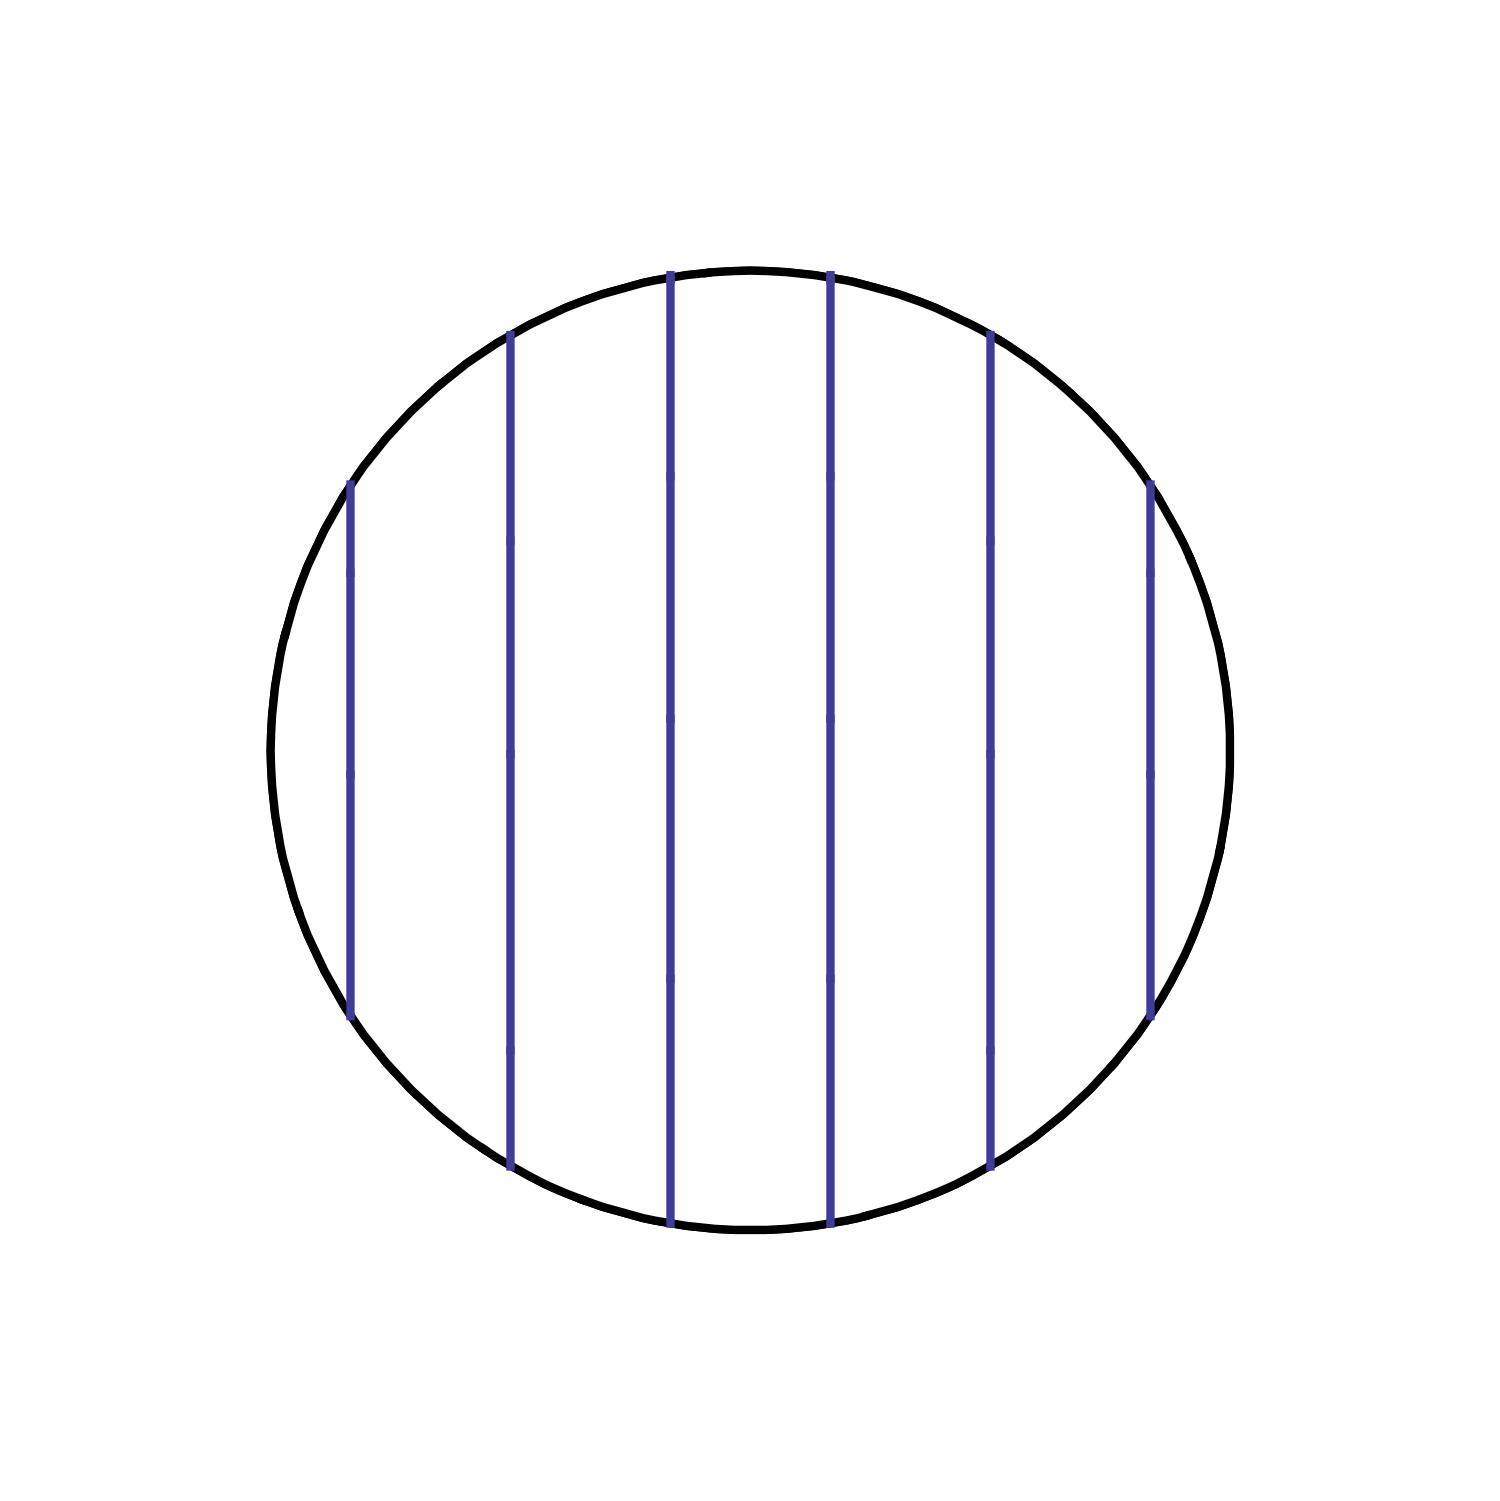
\includegraphics[width= 0.3\textwidth]{../A10tetel/Eb}}
%       \put(8.4,71){\tikz \draw[-latex,thick,blue] (0,0) -- (0,0.1);}
%       \put(32.8,71){\tikz \draw[-latex,thick,blue] (0,0) -- (0,0.1);}
%       \put(47.8,71){\tikz \draw[-latex,thick,blue] (0,0) -- (0,0.1);}
%       \put(62.6,71){\tikz \draw[-latex,thick,blue] (0,0) -- (0,0.1);}
%       \put(77.5,71){\tikz \draw[-latex,thick,blue] (0,0) -- (0,0.1);}
%       \put(93.0,71){\tikz \draw[-latex,thick,blue] (0,0) -- (0,0.1);}
%       \put(107.6,71){\tikz \draw[-latex,thick,blue] (0,0) -- (0,0.1);}
%       \put(131.8,71){\tikz \draw[-latex,thick,blue] (0,0) -- (0,0.1);}
%      \end{overpic}}
%     \hspace{6pt}
%     \subfloat[$\Dv(\rv)$ ($\ep_\text{k}<\ep_\text{g}$)\label{fig:10-2}]{\begin{overpic}[width= 0.3\textwidth]{../A10tetel/Db}
%       \put(8.4,71){\tikz \draw[-latex,thick,blue] (0,0) -- (0,0.1);}
%       \put(27.7,71){\tikz \draw[-latex,thick,blue] (0,0) -- (0,0.1);}
%       \put(37.8,71){\tikz \draw[-latex,thick,blue] (0,0) -- (0,0.1);}
%       \put(48.2,71){\tikz \draw[-latex,thick,blue] (0,0) -- (0,0.1);}
%       \put(58.8,71){\tikz \draw[-latex,thick,blue] (0,0) -- (0,0.1);}
%       \put(70.2,71){\tikz \draw[-latex,thick,blue] (0,0) -- (0,0.1);}
%       \put(81.5,71){\tikz \draw[-latex,thick,blue] (0,0) -- (0,0.1);}
%       \put(92.2,71){\tikz \draw[-latex,thick,blue] (0,0) -- (0,0.1);}
%       \put(102.7,71){\tikz \draw[-latex,thick,blue] (0,0) -- (0,0.1);}
%       \put(112.7,71){\tikz \draw[-latex,thick,blue] (0,0) -- (0,0.1);}
%       \put(131.8,71){\tikz \draw[-latex,thick,blue] (0,0) -- (0,0.1);}
%      \end{overpic}}
%     \hspace{6pt}
%     \subfloat[$\Ev_\text{dipól}(\rv)$ ($\ep_\text{k}<\ep_\text{g}$)\label{fig:10-3}]{\begin{overpic}[width= 0.3\textwidth]{../A10tetel/Pk}
%       \put(3.4,68){\tikz \draw[latex-,thick,blue] (0,0) -- (0,0.1);}
%       \put(35.3,68){\tikz \draw[latex-,thick,blue] (0,0) -- (0,0.1);}
%       \put(52.9,68){\tikz \draw[latex-,thick,blue] (0,0) -- (0,0.1);}
%       \put(70.4,68){\tikz \draw[latex-,thick,blue] (0,0) -- (0,0.1);}
%       \put(88,68){\tikz \draw[latex-,thick,blue] (0,0) -- (0,0.1);}
%       \put(105.2,68){\tikz \draw[latex-,thick,blue] (0,0) -- (0,0.1);}
%       \put(137,68){\tikz \draw[latex-,thick,blue] (0,0) -- (0,0.1);}      \put(60,106.3){\tikz\node[red] at (0,0) {\tiny $\pmb{\oplus}$};}
%       \put(68,106.3){\tikz\node[red] at (0,0) {\tiny $\pmb{\oplus}$};}
%       \put(89,98){\tikz\node[red] at (0,0) {\tiny $\pmb{\oplus}$};}
%       \put(39,98){\tikz\node[red] at (0,0) {\tiny $\pmb{\oplus}$};}
%       \put(60,21.7){\tikz\node[blue] at (0,0) {\tiny $\pmb{\ominus}$};}
%       \put(68,21.7){\tikz\node[blue] at (0,0) {\tiny $\pmb{\ominus}$};}
%       \put(89,30){\tikz\node[blue] at (0,0) {\tiny $\pmb{\ominus}$};}
%       \put(39,30){\tikz\node[blue] at (0,0) {\tiny $\pmb{\ominus}$};}
%      \end{overpic}}
%      %
%      \\
%      %
%      \subfloat[$\Ev(\rv)$ ($\ep_\text{k}>\ep_\text{g}$)\label{fig:10-4}]{\begin{overpic}[width= 0.3\textwidth]{../A10tetel/Dk}
%       \put(0,0){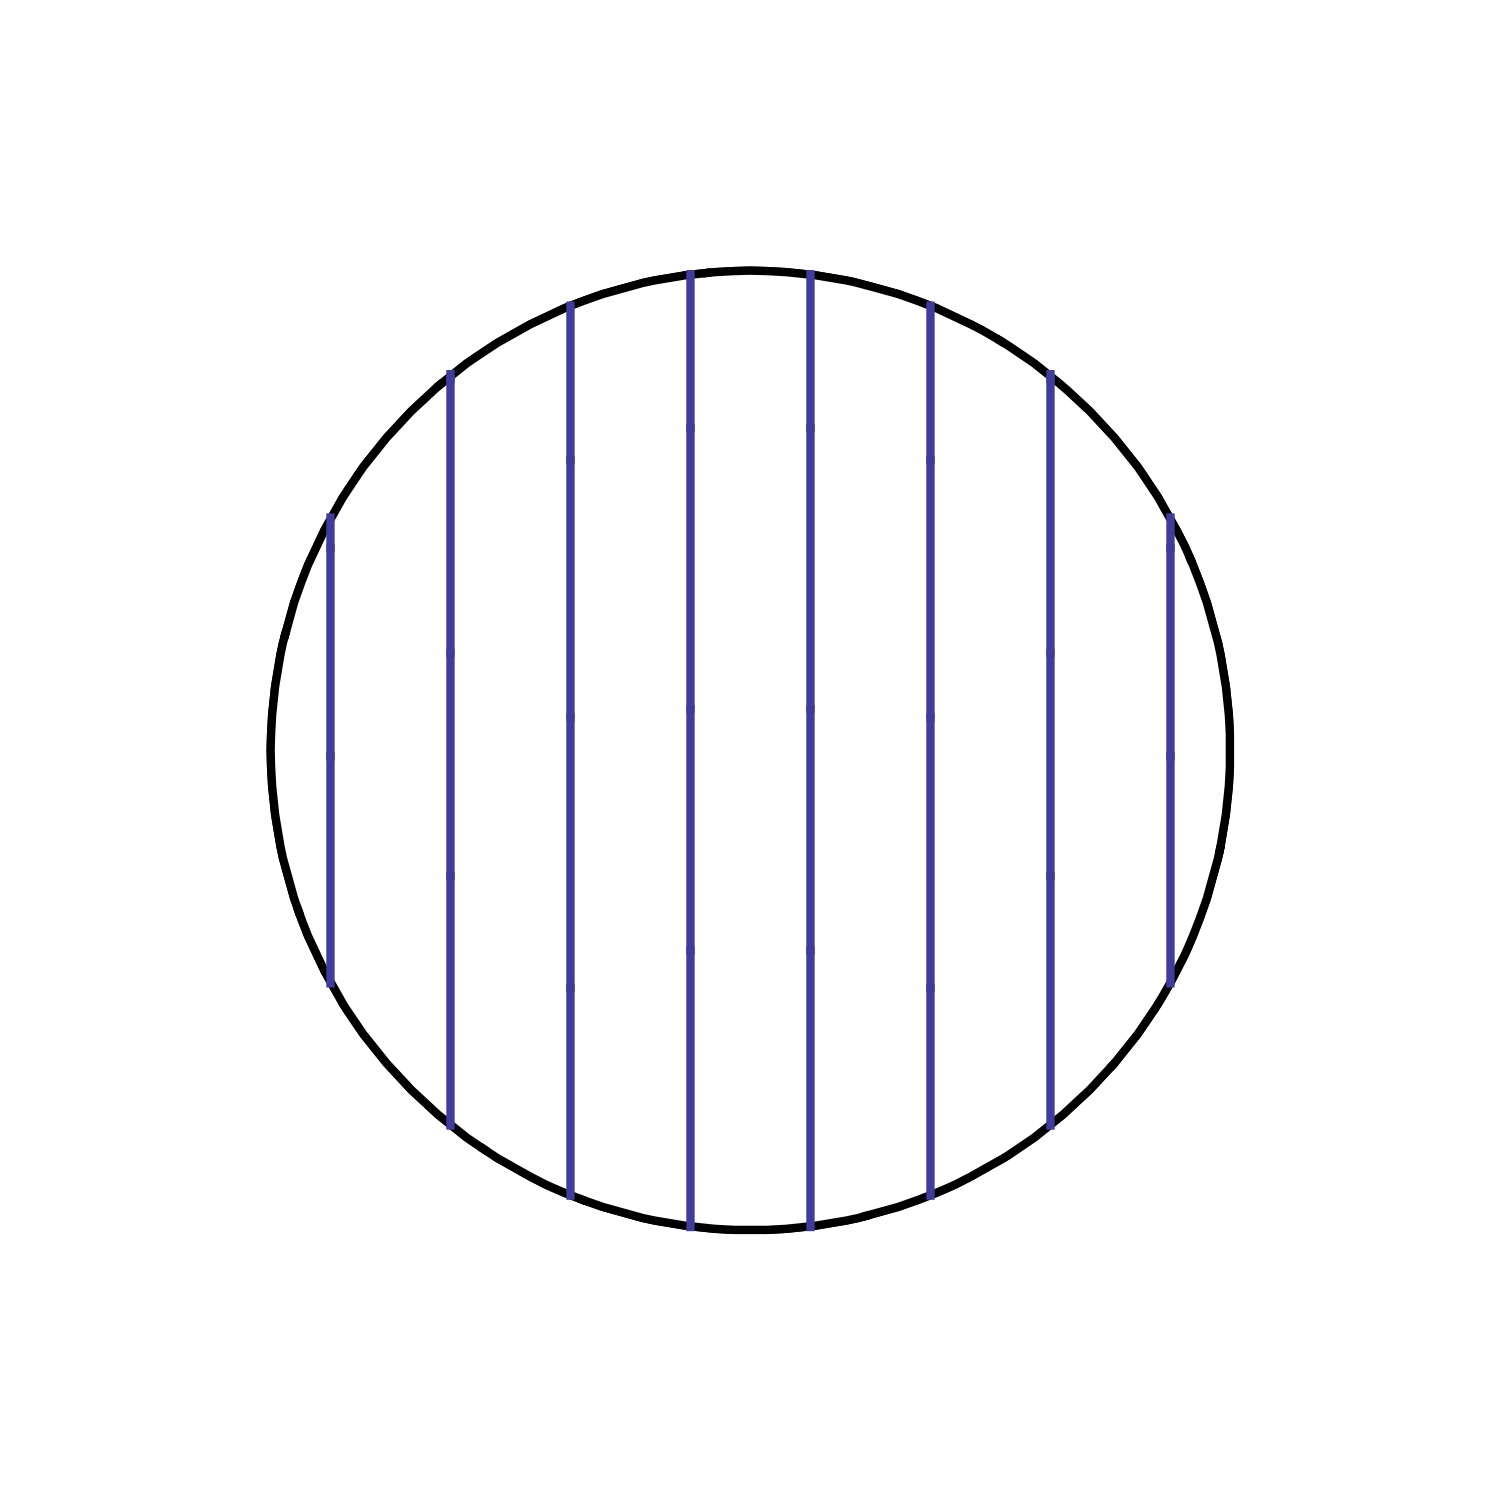
\includegraphics[width= 0.3\textwidth]{../A10tetel/Ek}}
%       \put(10.5,71){\tikz \draw[-latex,thick,blue] (0,0) -- (0,0.1);}
%       \put(20,71){\tikz \draw[-latex,thick,blue] (0,0) -- (0,0.1);}
%       \put(30.7,71){\tikz \draw[-latex,thick,blue] (0,0) -- (0,0.1);}
%       \put(42,71){\tikz \draw[-latex,thick,blue] (0,0) -- (0,0.1);}
%       \put(53.2,71){\tikz \draw[-latex,thick,blue] (0,0) -- (0,0.1);}
%       \put(64.4,71){\tikz \draw[-latex,thick,blue] (0,0) -- (0,0.1);}
%       \put(75.9,71){\tikz \draw[-latex,thick,blue] (0,0) -- (0,0.1);}
%       \put(87,71){\tikz \draw[-latex,thick,blue] (0,0) -- (0,0.1);}
%       \put(98.4,71){\tikz \draw[-latex,thick,blue] (0,0) -- (0,0.1);}
%       \put(109.6,71){\tikz \draw[-latex,thick,blue] (0,0) -- (0,0.1);}
%       \put(120.2,71){\tikz \draw[-latex,thick,blue] (0,0) -- (0,0.1);}
%       \put(130,71){\tikz \draw[-latex,thick,blue] (0,0) -- (0,0.1);}
%      \end{overpic}}
%     \hspace{6pt}
%     \subfloat[$\Dv(\rv)$ ($\ep_\text{k}>\ep_\text{g}$)\label{fig:10-5}]{\begin{overpic}[width= 0.3\textwidth]{../A10tetel/Dk}
%       \put(10.5,71){\tikz \draw[-latex,thick,blue] (0,0) -- (0,0.1);}
%       \put(20,71){\tikz \draw[-latex,thick,blue] (0,0) -- (0,0.1);}
%       \put(31.7,71){\tikz \draw[-latex,thick,blue] (0,0) -- (0,0.1);}
%       \put(51.2,71){\tikz \draw[-latex,thick,blue] (0,0) -- (0,0.1);}
%       \put(70.2,71){\tikz \draw[-latex,thick,blue] (0,0) -- (0,0.1);}
%       \put(89.2,71){\tikz \draw[-latex,thick,blue] (0,0) -- (0,0.1);}
%       \put(108.5,71){\tikz \draw[-latex,thick,blue] (0,0) -- (0,0.1);}
%       \put(120.2,71){\tikz \draw[-latex,thick,blue] (0,0) -- (0,0.1);}
%       \put(130,71){\tikz \draw[-latex,thick,blue] (0,0) -- (0,0.1);}
%      \end{overpic}}
%     \hspace{6pt}
%     \subfloat[$\Ev_\text{dipól}(\rv)$ ($\ep_\text{k}>\ep_\text{g}$)\label{fig:10-6}]{\begin{overpic}[width= 0.3\textwidth]{../A10tetel/Pk}
%       \put(3.4,71){\tikz \draw[-latex,thick,blue] (0,0) -- (0,0.1);}
%       \put(35.3,71){\tikz \draw[-latex,thick,blue] (0,0) -- (0,0.1);}
%       \put(52.9,71){\tikz \draw[-latex,thick,blue] (0,0) -- (0,0.1);}
%       \put(70.4,71){\tikz \draw[-latex,thick,blue] (0,0) -- (0,0.1);}
%       \put(88,71){\tikz \draw[-latex,thick,blue] (0,0) -- (0,0.1);}
%       \put(105.2,71){\tikz \draw[-latex,thick,blue] (0,0) -- (0,0.1);}
%       \put(137,71){\tikz \draw[-latex,thick,blue] (0,0) -- (0,0.1);}
%       \put(60,106.3){\tikz\node[blue] at (0,0) {\tiny $\pmb{\ominus}$};}
%       \put(68,106.3){\tikz\node[blue] at (0,0) {\tiny $\pmb{\ominus}$};}
%       \put(89,98){\tikz\node[blue] at (0,0) {\tiny $\pmb{\ominus}$};}
%       \put(39,98){\tikz\node[blue] at (0,0) {\tiny $\pmb{\ominus}$};}
%       \put(60,21.7){\tikz\node[red] at (0,0) {\tiny $\pmb{\oplus}$};}
%       \put(68,21.7){\tikz\node[red] at (0,0) {\tiny $\pmb{\oplus}$};}
%       \put(89,30){\tikz\node[red] at (0,0) {\tiny $\pmb{\oplus}$};}
%       \put(39,30){\tikz\node[red] at (0,0) {\tiny $\pmb{\oplus}$};}
%      \end{overpic}}
%     \caption{A homogén gömb körüli elektromos térerősség, eltolás és polarizációs tér, ha $\ep_\text{k}<\ep_\text{g}$ (első sor), illetve ha $\ep_\text{k}>\ep_\text{g}$ (második sor). Mivel $\Dv$ forrása a szabad töltések, ezért az itt folytonos. $\Ev$ forrása bármilyen töltés, és itt van felületi töltéssűrűség, ezért vannak olyan $\Ev$ vonalak, amelyek a felületen keletkeznek/végződnek.}
%     \end{figure}
    {\bf A szobák méretei:}
    \begin{figure}[ht!]
     \centering
     \begin{tikzpicture}
      \draw[thick] (0,0) -- node[left] {$4,99$\,m} (0,5.08);
      \draw[thick] (0,0) -- node[below] {$4,35$\,m} (4.35,0);
      \draw[thick] (4.35,5.08) -- node[right] {$5,08$\,m} (4.35,0);
      \draw[thick] (4.35,5.08) -- node[above] {$4,22$\,m} (0,5.08);
      \node at (2.155,2.54) {Nappali};
      
      \draw[thick,xshift=8cm] (0,0) -- node[left] {$5,04$\,m} (0,5.04);
      \draw[thick,xshift=8cm] (0,0) -- node[below] {$4,25$\,m} (4.25,0);
      \draw[thick,xshift=8cm] (4.25,5.04) -- node[right] {$5,04$\,m} (4.25,0);
      \draw[thick,xshift=8cm] (4.25,5.04) -- node[above] {$4,31$\,m} (0,5.04);
      \node[xshift=8cm] at (2.155,2.54) {Háló};
     \end{tikzpicture}
    \end{figure}
    
    {\bf A szobák alapterülete: }
    \al{
     A_\text{Nappali}
      &=\left(\frac{4,99\,m+5,08\,m}{2}\right)\cdot\left(\frac{4,22\,m+4,35\,m}{2}\right)
       =5,035\,m\cdot 4,285\,m
       \approx 21,6\,m^2\\
     A_\text{Háló}
      &=\left(\frac{5,04\,m+5,04\,m}{2}\right)\cdot\left(\frac{4,31\,m+4,25\,m}{2}\right)
       =5,04\,m\cdot 4,28\,m
       \approx 21,6\,m^2
    }
    
    {\bf A parketta mérete:} $45,5$\,cm$\times6,5$\,cm.

    
\end{document}